\documentclass[a4paper,12pt]{report}

\usepackage[english]{babel}
\usepackage[utf8]{inputenc}
\usepackage{indentfirst,setspace,subcaption}
\usepackage{amsmath,amssymb,graphicx,xcolor,url}
\usepackage{fancyhdr,tocbasic,titlesec,listings}
\usepackage[a4paper,margin=24mm]{geometry}
\usepackage[skip=10pt plus1pt, indent=20pt]{parskip}
\usepackage[colorlinks=true,allcolors=blue,urlcolor=magenta]{hyperref}

\renewcommand{\thesection}{\arabic{section}}

% Header and footer styling
\pagestyle{fancy}
\setlength{\headheight}{15pt}
\fancyhf{}
\fancyhead[R]{\nouppercase\rightmark\hfill~MOOCs report}
\fancyfoot[C]{\hfill\thepage\hfill}

% TOC styling
\DeclareTOCStyleEntry[
  indent=12pt,
  level=1
]{largetocline}{section}

% Title page data
\title{Massive Open Online Courses (MOOCs)\\Report}
\author{Ngo Nguyen The Khoa -- 23127065 -- 23CLC09}
\date{May 20, 2024}

\begin{document}

% Title page and TOC
\thispagestyle{empty}
\begin{titlepage}
	\begin{center}
		\makeatletter
		\newcommand{\HRule}{\rule{\linewidth}{0.4mm}}

		\textsc{\LARGE Vietnam National University,\\Ho Chi Minh City}\\[1.5cm]
		\textsc{\Large University of Science}\\[0.5cm]
		\textsc{\Large Faculty of Information Technology}\\[1.5cm]

		{\HRule}\\[1cm]
		{\huge \bfseries \@title}\\[0.5cm]
		{\HRule}\\[2cm]

		\textsc{\large CSC10004 -- Data Structures and Algorithms}\\[0.5cm]

		\vfill\vfill\vfill

		{\large \@author}\\[1.5cm]
		{\large \@date}
		\makeatother
	\end{center}
\end{titlepage}
\tableofcontents\thispagestyle{empty}

% Main content
\pagebreak
\section{Student's information}
\begin{itemize}
  \item \textbf{Name:} Ngo Nguyen The Khoa
  \item \textbf{Student ID:} 23127065
  \item \textbf{Class:} 23CLC09
  \item \textbf{Email:} \href{mailto:nntkhoa23@clc.fitus.edu.vn}{nntkhoa23@clc.fitus.edu.vn}
\end{itemize}

\pagebreak
\section{Courses' information}
\begin{itemize}
	\item \textbf{Google UX Design Professional Certificate} has 7 course series (\href{https://www.coursera.org/professional-certificates/google-ux-design}{more info}).
	\item The finish date of each course is shown as below
	      \begin{figure}[!ht]
		      \centering
		      
\includegraphics[width=0.5\textwidth]{imgs/FinishDay.png}
		      \caption{Course Finish Date}\label{fig:finish_date}
	      \end{figure}
	\item The date I enrolled each course is shown in the following table (export from Coursera):
	      \begin{figure}[!ht]
		      \centering
		      \begin{subfigure}{0.45\textwidth}
			      \centering
			      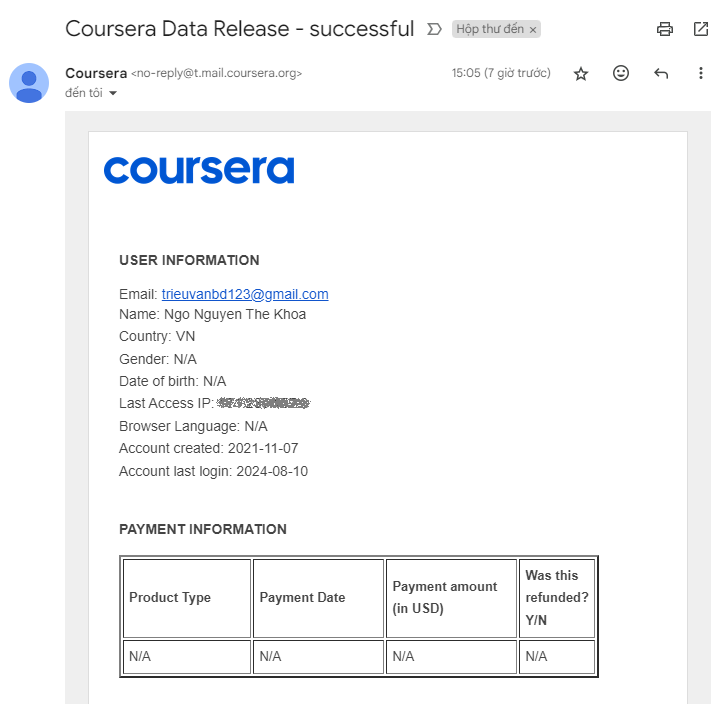
\includegraphics[width=\textwidth]{imgs/data-release-p1.png}
			      \caption{Enrollment Information P1}\label{fig:enrollment_info_p1}
		      \end{subfigure}
		      \hfill
		      \begin{subfigure}{0.45\textwidth}
			      \centering
			      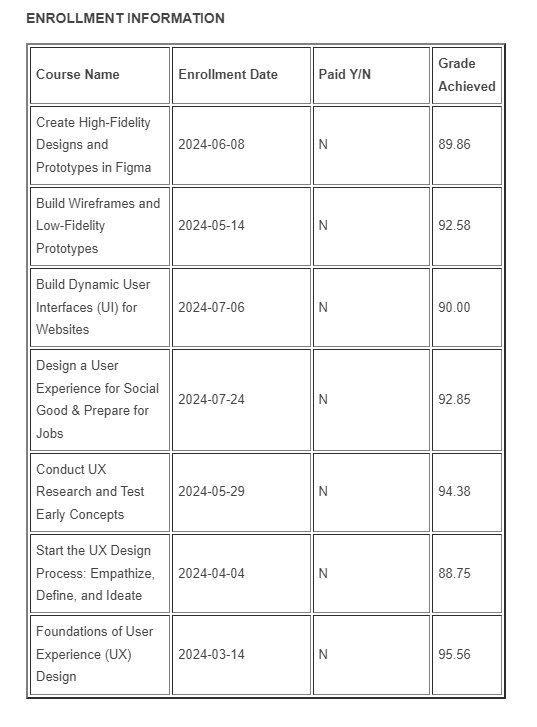
\includegraphics[width=\textwidth]{imgs/data-release-p2.png}
			      \caption{Enrollment Information P2}\label{fig:enrollment_info_p2}
		      \end{subfigure}

		      \caption{Enrollment Information}\label{fig:enrollment_info}
	      \end{figure}
\end{itemize}

\pagebreak
\subsection[Foundations of User Experience (UX) Design]{Course 1 -- Foundations of User Experience (UX) Design}
\subsubsection{Information}
\begin{itemize}
	\item \textbf{Course Name:} \href{https://www.coursera.org/learn/foundations-user-experience-design}{Foundations of User Experience (UX) Design}
	\item \textbf{Instructor:} \href{https://www.coursera.org/instructor/google-career-certificates}{Google Career Certificates}
	\item \textbf{Level:} Beginner
	\item \textbf{Enrolled on:} March 14, 2024
	\item \textbf{Finished on:} April 4, 2024
	\item \textbf{Grade Achieved:} 95.56\%
\end{itemize}

\subsubsection{Certificate}
\begin{flushleft}
	\begin{figure}[!ht]
		\centering
		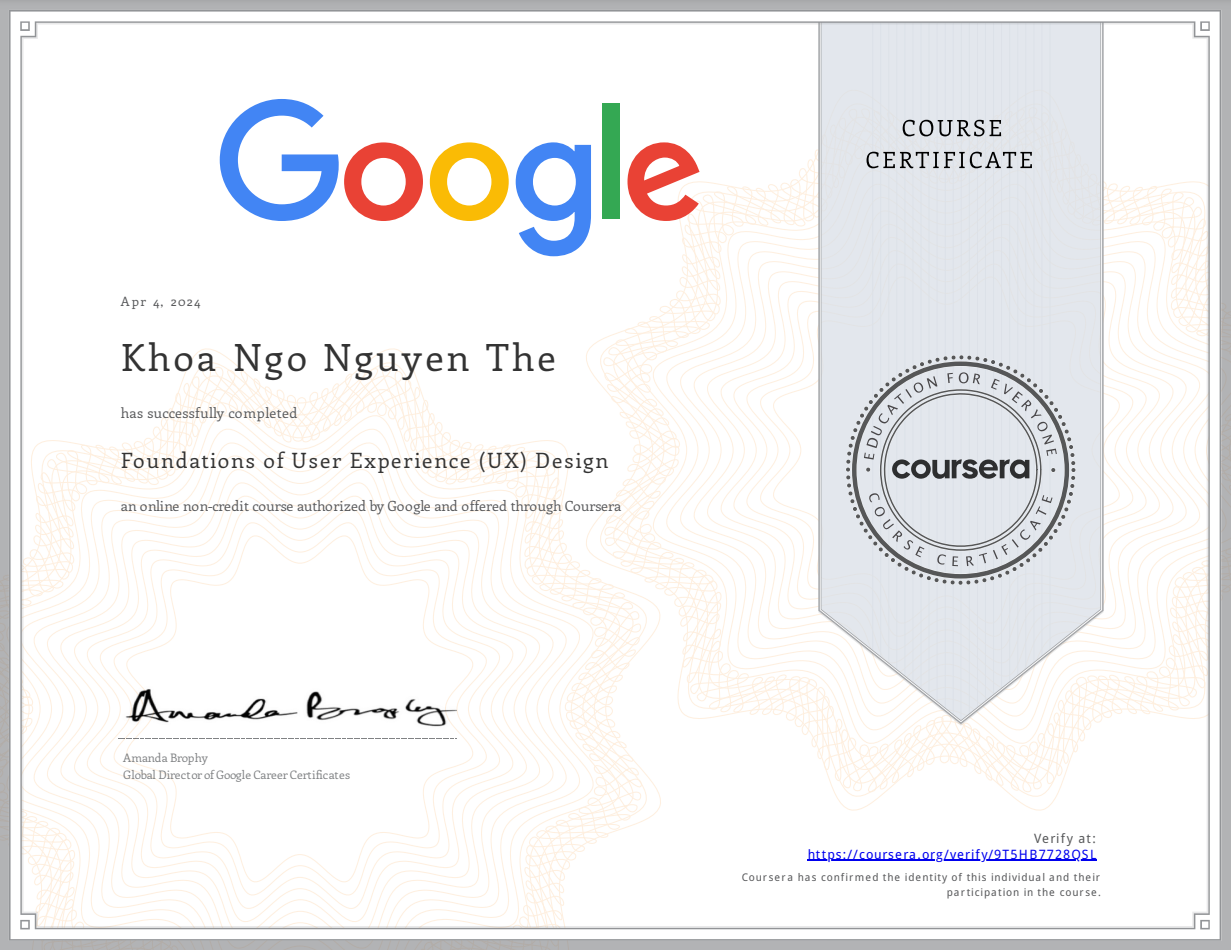
\includegraphics[width=0.85\textwidth]{imgs/Course1.png}
		\caption{Course 1 Certificate}
	\end{figure}

	Visit the online certificate for more info \href{https://www.coursera.org/account/accomplishments/verify/9T5HB7728QSL}{here}
\end{flushleft}

\subsubsection{Summary}
\begin{flushleft}
	What I have learned after completing this course:
	\begin{itemize}
		\item Identify common job responsibilities of entry-level UX designers and other teams I might work with.
		\item Understand foundational concepts in UX design, such as user-centered design, the design process, accessibility, and equity-focused design.
		\item Explain why design sprints are an important and useful part of a UX designer's work.
	\end{itemize}
\end{flushleft}

\subsubsection{Details}
\begin{flushleft}
	\begin{description}
		\item[Module 1:] Introducing User Experience Design
		      \begin{itemize}
			      \item I have been introduced to the world of UX and the factors that contribute to great user experience design. I have understand the job of a UX designer and teams that UX designers often work with.
			      \item I have also got to know more about the expectations of the Google UX Design Certificate.
		      \end{itemize}
		\item[Module 2:] Thinking like a UX Designer
		      \begin{itemize}
			      \item I have been introduced to user-centered design and one of the design frameworks that UX designers use on the job.
			      \item I have also learnt about design best practices, including the importance of inclusive design and accessibility when designing.
			      \item In addition, I have learnt how to think across platforms to design seamless user experiences.
		      \end{itemize}
		\item[Module 3:] Joining design sprints
		      \begin{itemize}
			      \item I have explored the world of design sprints, including the phases of a design sprint and how to plan and participate in one.
			      \item I have also learn about retrospectives, which is a way to constructively reflect on a design sprint and identify areas of improvement to implement next time.
		      \end{itemize}
		\item[Module 4:] Integrating research into the design process
		      \begin{itemize}
			      \item I have explored the role of research in the design process to help me better understand and empathize with users.
			      \item I have also learnt about the benefits and drawbacks of common UX research methods.
			      \item And, I have identified and accounted for biases that can arise when conducting research.
		      \end{itemize}
	\end{description}
\end{flushleft}

\pagebreak
\subsection[Start the UX Design Process: Empathize, Define, and Ideate]{Course 2 -- Start the UX Design Process: Empathize, Define, and Ideate}
\subsubsection{Information}
\begin{itemize}
	\item \textbf{Course Name:} \href{https://www.coursera.org/learn/start-ux-design-process}{Start the UX Design Process: Empathize, Define, and Ideate}
	\item \textbf{Instructor:} \href{https://www.coursera.org/instructor/google-career-certificates}{Google Career Certificates}
	\item \textbf{Level:} Beginner
	\item \textbf{Enrolled on:} April 4, 2024
	\item \textbf{Finished on:} April 30, 2024
	\item \textbf{Grade Achieved:} 88.75\%
\end{itemize}

\subsubsection{Certificate}
\begin{flushleft}
	\begin{figure}[!ht]
		\centering
		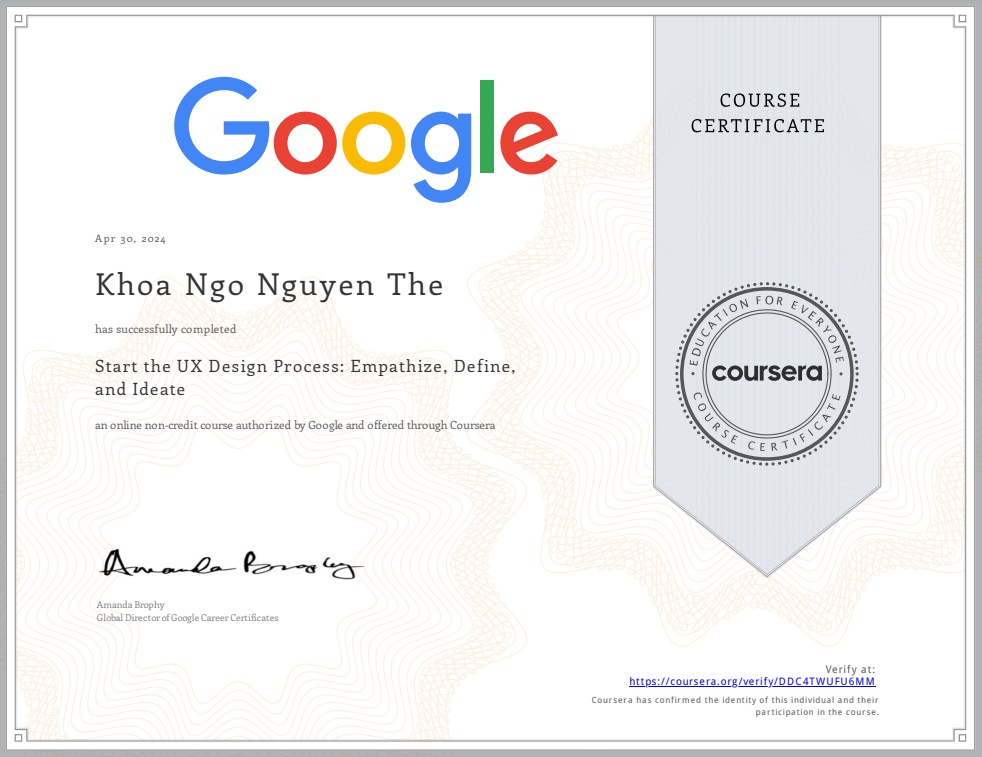
\includegraphics[width=0.85\textwidth]{imgs/Course2.png}
		\caption{Course 2 Certificate}
	\end{figure}

	Visit the online certificate for more info \href{https://www.coursera.org/account/accomplishments/verify/DDC4TWUFU6MM}{here}
\end{flushleft}

\subsubsection{Summary}
\begin{flushleft}
	What I have learned after completing this course:
	\begin{itemize}
		\item Empathize with users to understand their needs and pain points.
		\item Develop problem statements to define user needs.
		\item Generate ideas for possible solutions to user problems.
	\end{itemize}
\end{flushleft}

\subsubsection{Details}
\begin{flushleft}
	\begin{description}
		\item[Module 1:] Empathizing with users and defining pain points
		      \begin{itemize}
			      \item I have thought through the needs of my potential users to build empathy maps and create personas. These hands-on activities helped me understand user perspectives and pain points.
		      \end{itemize}
		\item[Module 2:] Creating user stories and user journey maps
		      \begin{itemize}
			      \item I have continued to empathize with users of the mobile app and crafted user stories and develop user journey maps.
			      \item I have also learnt about the importance of considering accessibility when empathizing with users.
		      \end{itemize}
		\item[Module 3:] Defining user problems
		      \begin{itemize}
			      \item I have moved from the empathize phase into the define phase of the design process.
			      \item To define the problem my designs will solve, I have built a problem statement, a hypothesis statement, and a value proposition.
			      \item In addition, I have explored how psychology and human factors influence design.
		      \end{itemize}
		\item[Module 4:] Ideating design solutions
		      \begin{itemize}
			      \item I have considered everything I've learnt about the users I'm designing for and the problems they're facing in order to brainstorm ideas for design solutions.
		      \end{itemize}
	\end{description}
\end{flushleft}

\pagebreak
\subsection[Build Wireframes and Low-Fidelity Prototypes]{Course 3 -- Build Wireframes and Low-Fidelity Prototypes}
\subsubsection{Information}
\begin{itemize}
	\item \textbf{Course Name:} \href{https://www.coursera.org/learn/wireframes-low-fidelity-prototypes}{Build Wireframes and Low-Fidelity Prototypes}
	\item \textbf{Instructor:} \href{https://www.coursera.org/instructor/google-career-certificates}{Google Career Certificates}
	\item \textbf{Level:} Beginner
	\item \textbf{Enrolled on:} May 14, 2024
	\item \textbf{Finished on:} May 29, 2024
	\item \textbf{Grade Achieved:} 92.58\%
\end{itemize}

\subsubsection{Certificate}
\begin{flushleft}
	\begin{figure}[!ht]
		\centering
		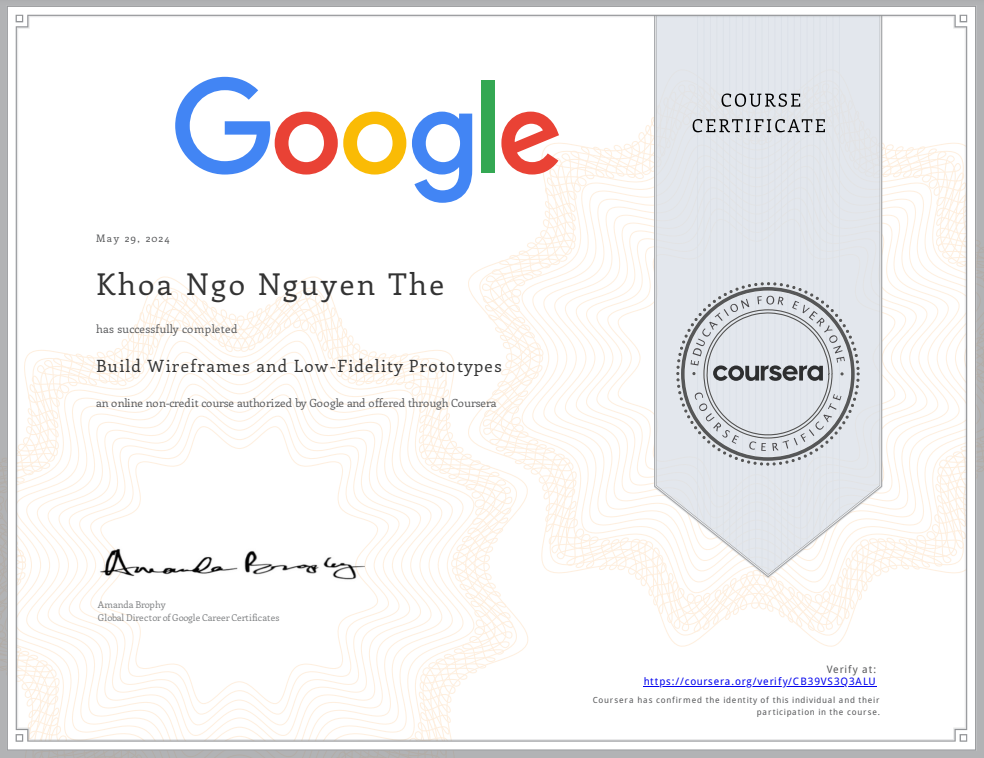
\includegraphics[width=0.85\textwidth]{imgs/Course3.png}
		\caption{Course 3 Certificate}
	\end{figure}

	Visit the online certificate for more info \href{https://www.coursera.org/account/accomplishments/verify/CB39VS3Q3ALU}{here}
\end{flushleft}

\subsubsection{Summary}
\begin{flushleft}
	What I have learned after completing this course:
	\begin{itemize}
		\item Create storyboards to come up with ideas about solutions to user needs.
		\item Create wireframes on paper and digitally in the design tool Figma.
		\item Build paper prototypes to create interactive designs.
		\item Design low-fidelity prototypes in Figma.
	\end{itemize}
\end{flushleft}

\subsubsection{Details}
\begin{flushleft}
	\begin{description}
		\item[Module 1:] Storyboarding and wireframing
		      \begin{itemize}
			      \item I have learnt how to use research findings to inform ideation during the design process.
			      \item I have created two types of storyboards: big picture and close-up.
			      \item I have drawn my first wireframes, and explored the benefits of wireframing.
		      \end{itemize}
		\item[Module 2:] Creating paper and digital wireframes
		      \begin{itemize}
			      \item I have learnt Figma about how to best use their tool.
			      \item I have applied Gestalt Principles, like similarity, proximity, and common region, to my wireframes.
		      \end{itemize}
		\item[Module 3:] Building low-fidelity prototypes
		      \begin{itemize}
			      \item I have transition to a digital low-fidelity prototype in Figma.
			      \item I have explored ways to recognize potential bias in my designs and learnt how to avoid deceptive patterns.
		      \end{itemize}
	\end{description}
\end{flushleft}

\pagebreak
\subsection[Conduct UX Research and Test Early Concepts]{Course 4 -- Conduct UX Research and Test Early Concepts}
\subsubsection{Information}
\begin{itemize}
	\item \textbf{Course Name:} \href{https://www.coursera.org/learn/conduct-ux-research}{Conduct UX Research and Test Early Concepts}
	\item \textbf{Instructor:} \href{https://www.coursera.org/instructor/google-career-certificates}{Google Career Certificates}
	\item \textbf{Level:} Beginner
	\item \textbf{Enrolled on:} May 29, 2024
	\item \textbf{Finished on:} June 8, 2024
	\item \textbf{Grade Achieved:} 94.38\%
\end{itemize}

\subsubsection{Certificate}
\begin{flushleft}
	\begin{figure}[!ht]
		\centering
		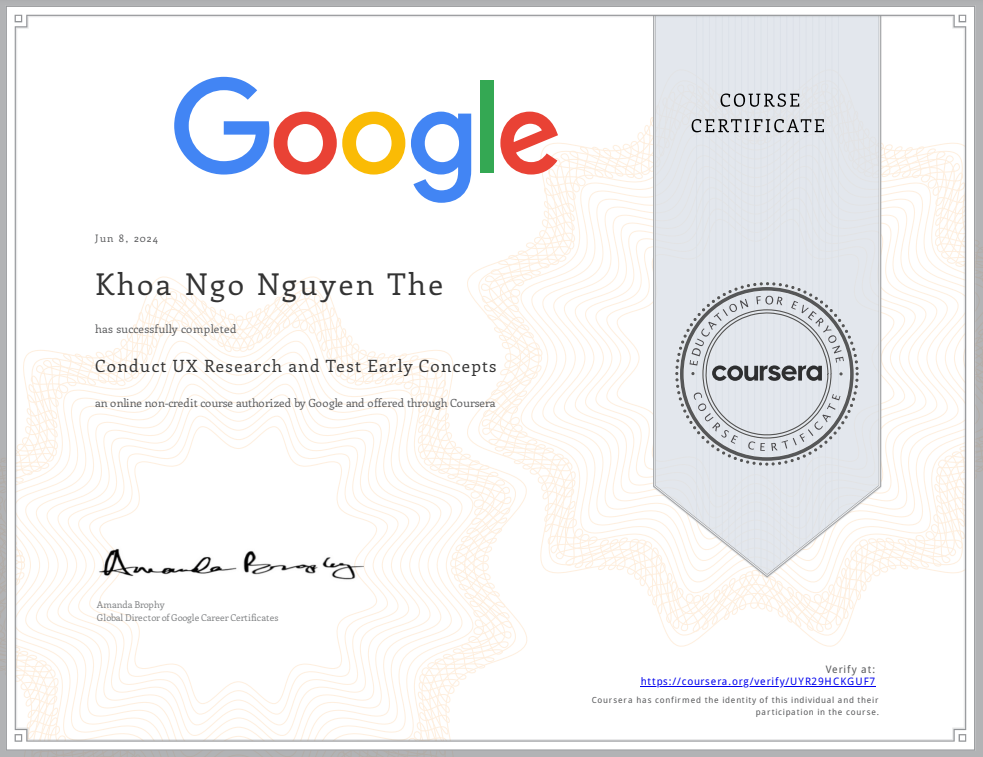
\includegraphics[width=0.85\textwidth]{imgs/Course4.png}
		\caption{Course 4 Certificate}
	\end{figure}

	Visit the online certificate for more info \href{https://www.coursera.org/account/accomplishments/verify/UYR29HCKGUF7}{here}
\end{flushleft}

\subsubsection{Summary}
\begin{flushleft}
	What I have learned after completing this course:
	\begin{itemize}
		\item Plan and conduct moderated and unmoderated usability studies.
		\item Synthesize observations from usability studies and come up with insights.
		\item Share research methodology and insights using persuasive presentation skills.
		\item Modify low-fidelity designs based on research insights.
	\end{itemize}
\end{flushleft}

\subsubsection{Details}
\begin{flushleft}
	\begin{description}
		\item[Module 1:] Planning UX research studies
		      \begin{itemize}
			      \item I have learnt how to plan a UX research study.
			      \item I have explored each of mentioned seven elements in detail, and I have created my own research plan to test the designs I developed in the previous course (Course 3).
			      \item I have also learnt how to respect user privacy and data when conducting UX research.
		      \end{itemize}
		\item[Module 2:] Conducting research with usability studies
		      \begin{itemize}
			      \item I have conducted a usability study, which is a research method that assesses how easy it is for participants to complete core tasks in a design.
			      \item I have also explored how to reduce bias and be inclusive when conducting usability studies.
			      \item I have taken notes while observing participants in a usability study.
		      \end{itemize}
		\item[Module 3:] Analyzing and synthesizing research results
		      \begin{itemize}
			      \item I have analyzed and synthesized all of the feedback from my research.
			      \item I have gathered data and observations in one place, organized the data using an affinity diagram, found themes, and come up with actionable insights.
		      \end{itemize}
		\item[Module 4:] Sharing research insights for better designs
		      \begin{itemize}
			      \item I have learnt techniques for presenting insights to various audiences, and improved my presentation skills to grab my audience's attention.
			      \item I have iterated on my designs, which means making revisions to create new-and-improved designs, based on insights from my research.
		      \end{itemize}
	\end{description}
\end{flushleft}

\pagebreak
\subsection[Create High-Fidelity Designs and Prototypes in Figma]{Course 5 -- Create High-Fidelity Designs and Prototypes in Figma}
\subsubsection{Information}
\begin{itemize}
	\item \textbf{Course Name:} \href{https://www.coursera.org/learn/high-fidelity-designs-prototype}{Create High-Fidelity Designs and Prototypes in Figma}
	\item \textbf{Instructor:} \href{https://www.coursera.org/instructor/google-career-certificates}{Google Career Certificates}
	\item \textbf{Level:} Beginner
	\item \textbf{Enrolled on:} June 8, 2024
	\item \textbf{Finished on:} July 6, 2024
	\item \textbf{Grade Achieved:} 89.86\%
\end{itemize}

\subsubsection{Certificate}
\begin{flushleft}
	\begin{figure}[!ht]
		\centering
		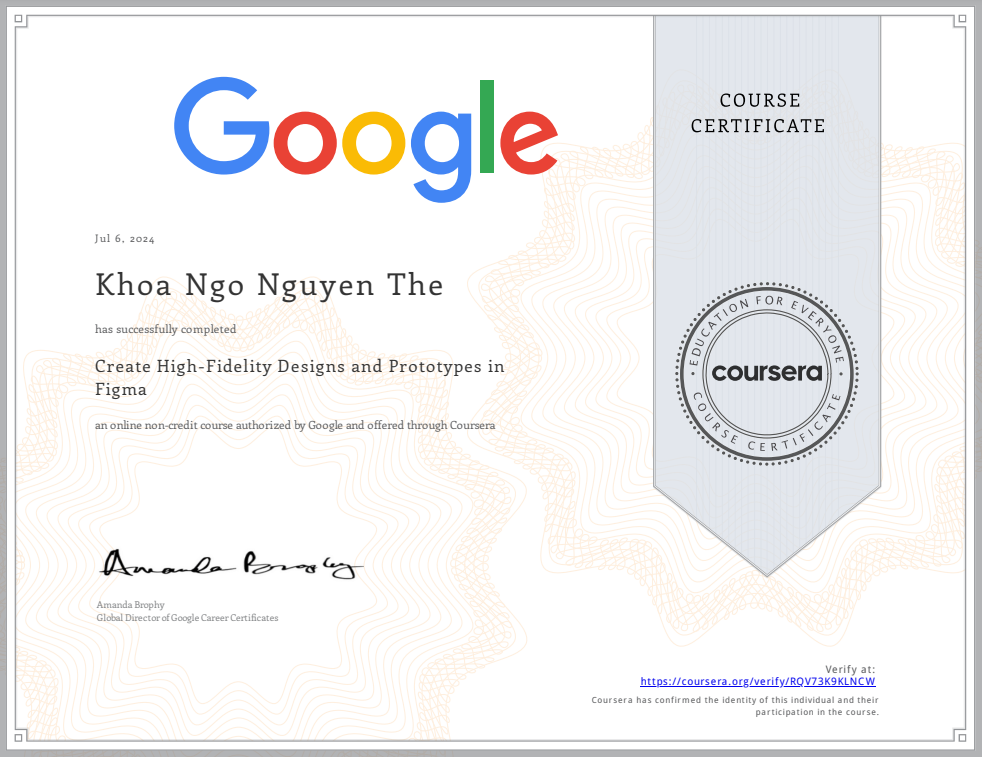
\includegraphics[width=0.85\textwidth]{imgs/Course5.png}
		\caption{Course 5 Certificate}
	\end{figure}

	Visit the online certificate for more info \href{https://www.coursera.org/account/accomplishments/verify/RQV73K9KLNCW}{here}
\end{flushleft}

\subsubsection{Summary}
\begin{flushleft}
	What I have learned after completing this course:
	\begin{itemize}
		\item Build mockups and high-fidelity prototypes in the design tool Figma.
		\item Define and apply common visual design elements and principles.
		\item Demonstrate how design systems can be used to organize, standardize, and enhance designs.
		\item Understand the role of design critique sessions and feedback while iterating on designs.
	\end{itemize}
\end{flushleft}

\subsubsection{Details}
\begin{flushleft}
	\begin{description}
		\item[Module 1:] Starting to create mockups
		      \begin{itemize}
			      \item I have used visual design elements, like typography, color, and iconography to create mockups.
			      \item I have applied visual design learnings to build on the mobile app designs I've been working on throughout the certificate program.
		      \end{itemize}
		\item[Module 2:] Applying visual design principles to mockups
		      \begin{itemize}
			      \item I have used visual design principles to refine mockups and emphasis to guide users to the most important parts of a page.
			      \item I have applied hierarchy, scale, and proportion to organize the elements on each page of my app.
			      \item I have revisited Gestalt Principles, like similarity, proximity, and common region, to help users interpret my designs easily.
		      \end{itemize}
		\item[Module 3:] Exploring design systems
		      \begin{itemize}
			      \item I have known the parts of a design system, as well as the benefits of using a design system.
			      \item I have examined various companies' design systems, and had an opportunity to use them in my own mockups.
			      \item I have also learnt how to use and create sticker sheets in Figma.
		      \end{itemize}
		\item[Module 4:] Creating high-fidelity prototypes
		      \begin{itemize}
			      \item I have turned my mockups into a prototype that's ready for testing.
			      \item I have explored two new concepts, gestures and motion, which can help enrich the user experience and increase the usability of prototypes.
		      \end{itemize}
		\item[Module 5:] Testing and iterating on designs
		      \begin{itemize}
			      \item I have conducted a usability study to test my high-fidelity prototype of a mobile app and learnt how to hand off designs to engineers for production.
			      \item I have analyzed the feedback I received to come up with actionable insights and iterate on my designs.
			      \item I have turned everything I learnt about user research, ideation, wireframes, designs, and prototypes into a case study for my professional UX portfolio.
		      \end{itemize}
	\end{description}
\end{flushleft}

\pagebreak
\subsection[Build Dynamic User Interfaces (UI) for Websites]{Course 6 -- Build Dynamic User Interfaces (UI) for Websites}
\subsubsection{Information}
\begin{itemize}
	\item \textbf{Course Name:} \href{https://www.coursera.org/learn/responsive-web-design-adobe-xd}{Build Dynamic User Interfaces (UI) for Websites}
	\item \textbf{Instructor:} \href{https://www.coursera.org/instructor/google-career-certificates}{Google Career Certificates}
	\item \textbf{Level:} Beginner
	\item \textbf{Enrolled on:} July 6, 2024
	\item \textbf{Finished on:} July 29, 2024
	\item \textbf{Grade Achieved:} 90.00\%
\end{itemize}

\subsubsection{Course is done}
\begin{figure}[!ht]
	\centering
	\begin{subfigure}{0.75\textwidth}
		\centering
		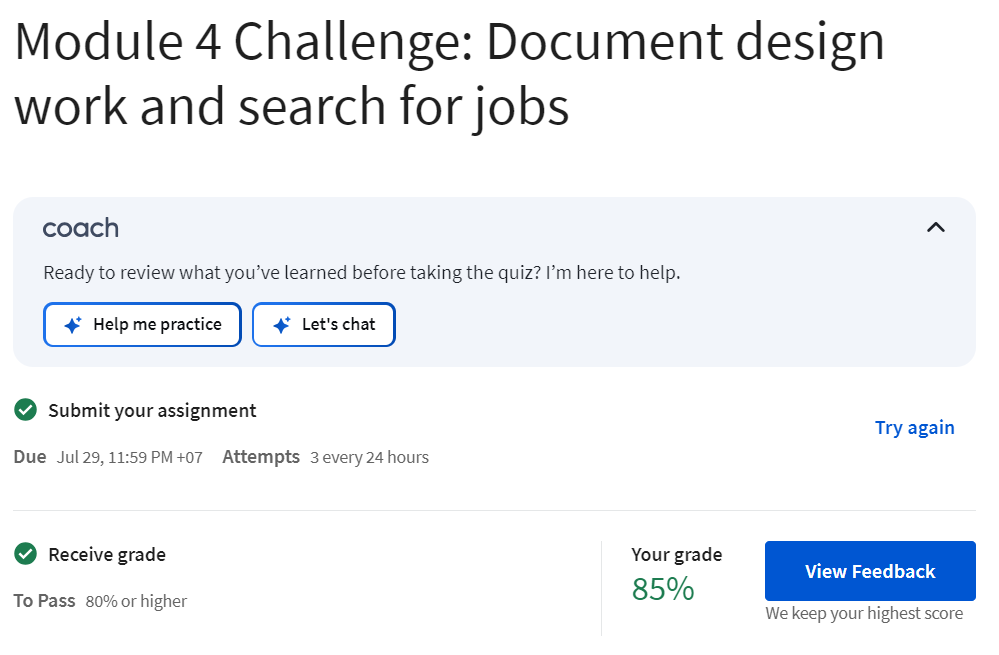
\includegraphics[width=\textwidth]{imgs/Course6-M4.png}
	\end{subfigure}
	\hfill
	\begin{subfigure}{0.75\textwidth}
		\centering
		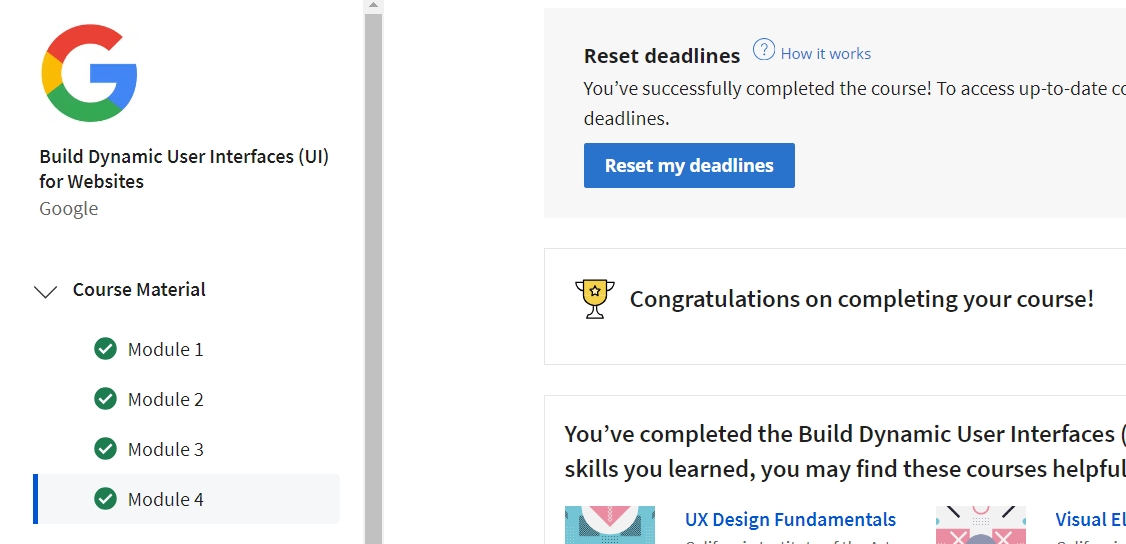
\includegraphics[width=\textwidth]{imgs/Course6-Done.png}
	\end{subfigure}
	\caption{Course 6 - Done}
\end{figure}

\subsubsection{Summary}
\begin{flushleft}
	What I have learned after completing this course:
	\begin{itemize}
		\item Apply each step of the UX design thinking framework (empathize, define, ideate, prototype, test) to create a dynamic website.
		\item Plan information architecture and sitemaps for website designs.
		\item Apply common layouts for web pages.
		\item Complete a design project and include it in your professional UX portfolio.
	\end{itemize}
\end{flushleft}

\subsubsection{Details}
\begin{flushleft}
	\begin{description}
		\item[Module 1:] Plan a responsive website
		      \begin{itemize}
			      \item I have completed the empathize and define phases.
		      \end{itemize}
		\item[Module 2:] Create and test prototypes
		      \begin{itemize}
			      \item I have learnt how to build a low-fidelity prototype.
			      \item I have made changes to my low-fidelity designs based on insights from my research.
		      \end{itemize}
		\item[Module 3:] Participating in design critique sections
		      \begin{itemize}
			      \item I have explored common website layouts, and created paper wireframes.
			      \item I have known a few elements and components that are commonly used in responsive website design.
			      \item I have updated and refined my wireframes to enhance accessibility.
		      \end{itemize}
		\item[Module 4:] Document design work and search for jobs
		      \begin{itemize}
			      \item I have learnt how to prepare and handoff designs to engineers, who will build the final product.
			      \item I have also added a case study to my professional UX portfolio featuring my responsive website designs.
			      \item I have learnt tips and tricks to scan job postings, and created a compelling resume that highlights my new UX skills.
		      \end{itemize}
	\end{description}
\end{flushleft}

\pagebreak
\subsection[Design a User Experience for Social Good \& Prepare for Jobs]{Course 7 -- Design a User Experience for Social Good \& Prepare for Jobs}
\subsubsection{Information}
\begin{itemize}
	\item \textbf{Course Name:} \href{https://www.coursera.org/learn/ux-design-jobs}{Design a User Experience for Social Good \& Prepare for Jobs}
	\item \textbf{Instructor:} \href{https://www.coursera.org/instructor/google-career-certificates}{Google Career Certificates}
	\item \textbf{Level:} Beginner
	\item \textbf{Enrolled on:} July 24, 2024
	\item \textbf{Finished on:} August 16, 2024
	\item \textbf{Grade Achieved:} 92.85\%
\end{itemize}

\subsubsection{Course is done}
\begin{figure}[!ht]
	\centering
	\begin{subfigure}{0.75\textwidth}
		\centering
		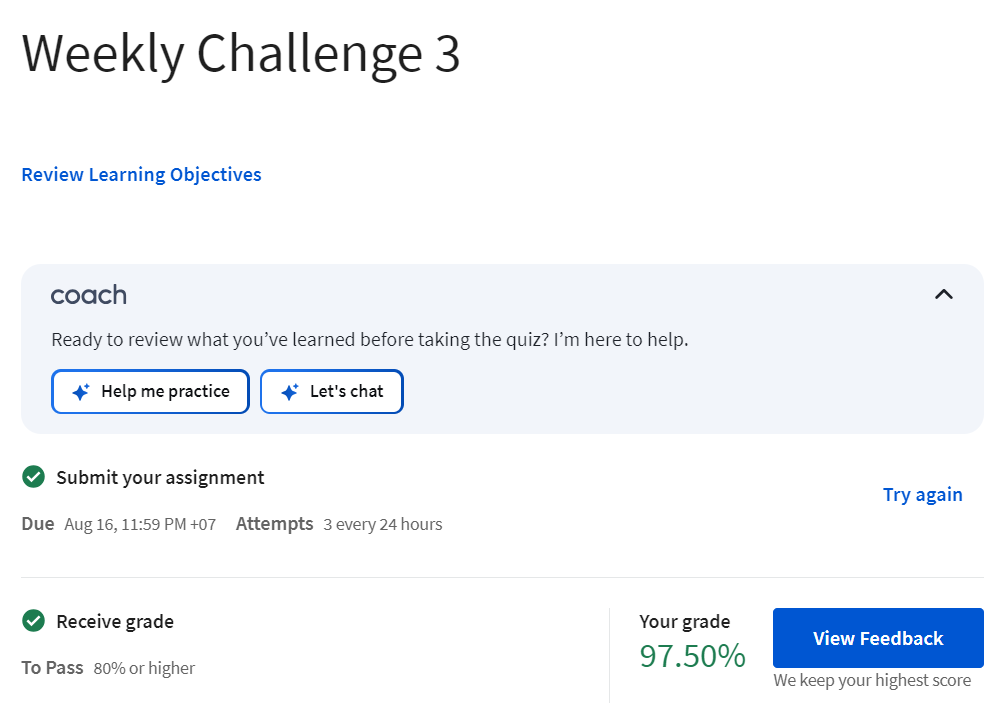
\includegraphics[width=\textwidth]{imgs/Course7-M3.png}
	\end{subfigure}
	\hfill
	\begin{subfigure}{0.75\textwidth}
		\centering
		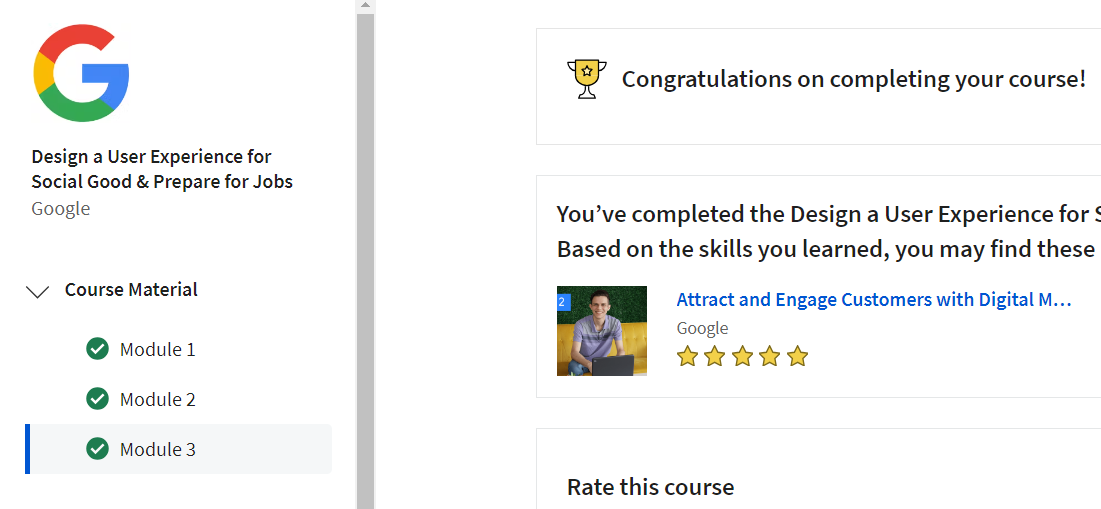
\includegraphics[width=\textwidth]{imgs/Course7-Done.png}
	\end{subfigure}
	\caption{Course 7 - Done}
\end{figure}

\subsubsection{Summary}
\begin{flushleft}
	What I have learned after completing this course:
	\begin{itemize}
		\item Apply each step of the UX design thinking framework (empathize, define, ideate, prototype, test) to create a  project focused on social good.
		\item Build wireframes, mockups, and low-fidelity and high-fidelity prototypes for a dedicated mobile app and a responsive website.
		\item Prepare to successfully interview for an entry-level UX design job.
		\item Determine if freelance design work is a good career fit.
	\end{itemize}
\end{flushleft}

\subsubsection{Details}
\begin{flushleft}
	\begin{description}
		\item[Module 1:] Design for social good and strengthen your portfolio
		      \begin{itemize}
			      \item I have designed a dedicated mobile app and a responsive website focused on social good that showcases everything I've learned in the program.
		      \end{itemize}
		\item[Module 2:] Build a professional presence
		      \begin{itemize}
			      \item I have created a portfolio to showcase my upcoming work.
			      \item I have also learnt about the importance of having a personal brand and building an online presence.
		      \end{itemize}
		\item[Module 3:] Finding a UX job
		      \begin{itemize}
			      \item I have made final adjustments to my portfolio to ensure it's ready to share in job applications.
			      \item I have examined the UX design interview process and develop strategies to succeed in various types of interview.
		      \end{itemize}
	\end{description}
\end{flushleft}

% Bibliography
% \pagebreak
% \bibliography{bilbs/refs}
% \bibliographystyle{ieeetr}

\end{document}